\documentclass[a4j,10pt,oneside,openany]{jsbook}
%
\usepackage{amsmath,amssymb}
\usepackage{bm}
\usepackage[dvipdfm]{graphicx}
\usepackage{wrapfig}
\usepackage{ascmac}
\usepackage{makeidx}
%
\makeindex
%
\newcommand{\diff}{\mathrm{d}}  %微分記号
\newcommand{\divergence}{\mathrm{div}\,}  %ダイバージェンス
\newcommand{\grad}{\mathrm{grad}\,}  %グラディエント
\newcommand{\rot}{\mathrm{rot}\,}  %ローテーション
%
\setlength{\textwidth}{\fullwidth}
\setlength{\textheight}{44\baselineskip}
\addtolength{\textheight}{\topskip}
\setlength{\voffset}{-0.6in}
%
\title{{\Huge \textbf{修士論文}}}
\author{工学系研究科電気系工学専攻修士2年\\学籍番号:37-176484\\ 氏名:松崎博貴\\ 指導教官:小野寺宏}
\date{\today}
\begin{document}
%
%
\maketitle
\frontmatter
\tableofcontents
%
%
\mainmatter
\chapter{はじめに}
近年になって医療データが蓄積されるシステムができてきいる。医療画像をコンピューター上に取り込むようになってから、自動で解析するシステムを構築してきた。今までは、専門医が診断を行う場合は、判断が主観的であること、ミスをする可能性があること、専門化同士でも意見が異なること、実際の臨床現場で医師はたくさんの画像を処理しなくてはいけないので、1枚にかけられる時間が限られていることから、機械による診断支援システムが必要とされている。既存の機械によるルールベースによるシステムでは解析ルール人にバイアスがかかっているということや、画像認識の著しい精度向上があるディープラーニングを利用した方法によって解析する方法に注目されている。またコンピュータの計算性能と、ビッグデータである医療画像を処理する能力が向上した背景と重なって、現在は機械学習による医療画像解析の研究が盛り上がりを見せている。第1章ではディープラーニングの基本的な原理と手法の紹介を行う。

\chapter{ディープラーニングによる画像認識}
\section{ILSVC2012}
ディープラーニングが注目を受けることになったのは、2012の画像認識コンペティションであるILSVCでHintonがAlexNetというDeepLearningの手法で他のチームを圧倒する精度を出したことが始まりである。
\section{ディープラーニングができること}
画像処理におけるディープラーニングができることは、画像から(1)カテゴリ分けをすること、(2)物体を検出すること、(3)物体のセグメンテーションをすることである。医療画像で例えるならば、画像から、癌があるか正常化を見分けることが(1)カテゴリ分けであり、癌がある場所を検出することが(2)物体検出であり、癌の部分をセグメンテーションすることが(3)物体のセグメンテーションになる。
\section{ディープラーニングの原理}
ディープラーニングは、その名の通り、今までのニューラルネットワークよりも層が深くなっている。この層の深さが、より複雑な特徴を抽出することができる。層の深さはモデル設計でチューニングしていく必要があり、上述のAlexNetは8層のネットワークであった。しかし、ネットワークの層は深くなっていき、現在では152層のResNetというものがILSVC2015でもっとも精度が良く、人間の認識精度を超えている。ディープラーニングによる学習方法について、畳み込みニューラルネットワーク(Convolutional Neural Network : CNN)を利用する。入力する画像に対して小さなサイズ(3×3など)のフィルターを畳み込み計算をする。このフィルターの値を学習することがディープラーニングの学習である。フィルターの数も設計する必要がある。学習については、誤差逆伝播法を利用する。ディープラーニングの出力結果と正解との比較をした時に、どれだけ正解から離れているかを評価する誤差関数を使って、その誤差関数が小さくなるように、フィルターの重みを変更する時に勾配降下法を使う。
\section{ディープラーニングによる2D医療画像認識}
ディープラーニングを利用して2次元の医療画像の解析について、研究動向を調査した。画像のクラス分けについては、皮膚癌の種類が757種類を細かい違いまで識別するように学習する。学習方法はInception v3というネットワークを利用している。これは22層の畳み込みニューラルネットワークである。またこのネットワークは皮膚癌の識別タスクを学習する前に、IMageNetというILSVCでも使っている一般物体画像を使って事前にネットワークの重みの初期値を決めることによって、精度が向上させる。これを転移学習(Transfer Learning)と呼ばれている。そして学習した結果を評価するときに医療画像の場合は、PrecisionとRecallを識別性能の評価指数として使う。\[ Precision = \frac{TP}{TP+FP}\hspace{10mm} Recall = \frac{TP}{TP+FN} \]ここで使ったTP(True Positive)は真の結果が正である時に予測も正であるという意味であるTN(True Negative)は真の結果が正で予測が負である場合である。同様にFP(False Positive)真の結果が負で予測も負、FN(False Negative)真の結果が負で予測は正である。\\
2016年に行われたCAMELYON16という乳がんの転移を調べるシステムのコンペティションでは、7人の医師の成績を上回っていることが報告されてている。
\section{ディープラーニングによる3D医療画像認識}
\section{3D医療画像認識の必要性と課題}
ディープラーニングを医療画像に応用するコンペティションが世界で行われているが、その半数が3D医療画像の解析になっているほど需要が高まっている。その理由は、現在解決しなくてはならない課題があるからである。まずは2次元画像と違って、処理するべきデータが大きいということである。そのため学習するパラメータをなるべく少なくする工夫がされている。また3次元画像には、動画または、ボリューム画像があるが、2次元画像とその深さ方向(動画であれば、時間方向)には異方性があることから、機械学習の方法に工夫が必要になる。今まで考案されている手法として、2DCNNを拡張した3DCNN、またCNNと時系列解析でよく用いられるLSTMを組み合わせた手法と、LSTM内部にCNNを組み込んだ手法、それらをすべて組み合わせた手法が考案されいる。LSTMの研究も盛んに行われているため、その改良モデルが数多く存在する。特に、LSTMの学習効率を上げたGRU(Gated Linear Unit)や、順方向だけでなく逆方向の時系列も計算に入れるBiLSTMが時系列解析の精度向上になっている報告がある。
\subsection{RNN, LSTMとその派生形}
\begin{figure}[h]
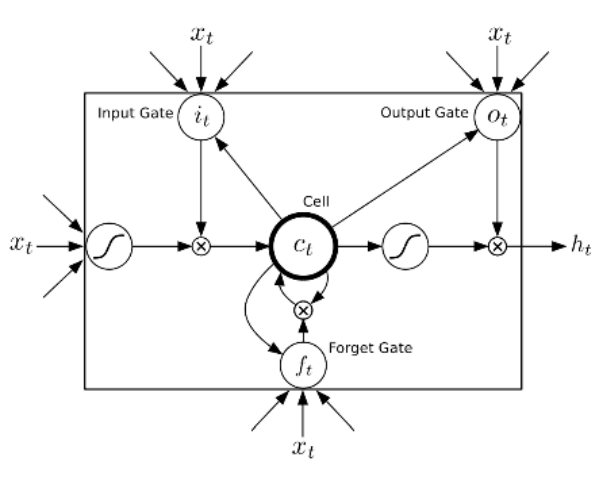
\includegraphics[width=10cm]{img/lstm.png}
\end{figure}

\begin{eqnarray}
  i_t & = & \sigma(W_{xi} x_t + W_{hi} h_{t-1} + W_{ci} c_{t-1} + b_i) \\
  f_t & = & \sigma(W_{xf} x_t + W_{hf} h_{t-1} + W_{cf} c_{t-1} + b_f ) \\
  c_t & = & f_t c_{t-1} + i_t tanh(W_{xc} x_t + W_{hc} h_{t-1} + b_c) \\
  o_t & = & \sigma(W_{xo} x_t + W_{ho} h_{t-1} + W_{co} c_t + b_o) \\
  h_t & = & o_t tanh(c_t) 
\end{eqnarray}

\subsection{3D CNNとStacked Convolution}
2次元画像が深さ方向に連続している3次元画像の特徴を抽出するために、2次元のCNNを拡張して、3次元のカーネルを使って畳み込みを行う、3DCNNを利用した手法がある。

\begin{figure}[h]
\centering
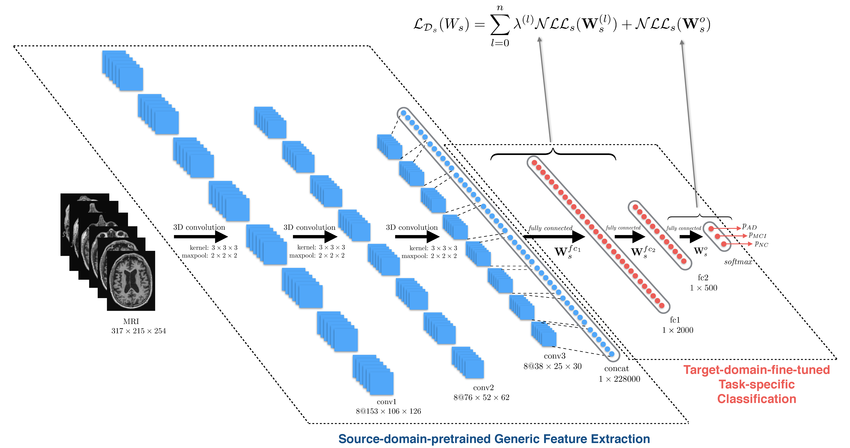
\includegraphics[width=0.7\linewidth]{img/3d_cnn.png}
\end{figure}


\begin{figure}[h]
\centering
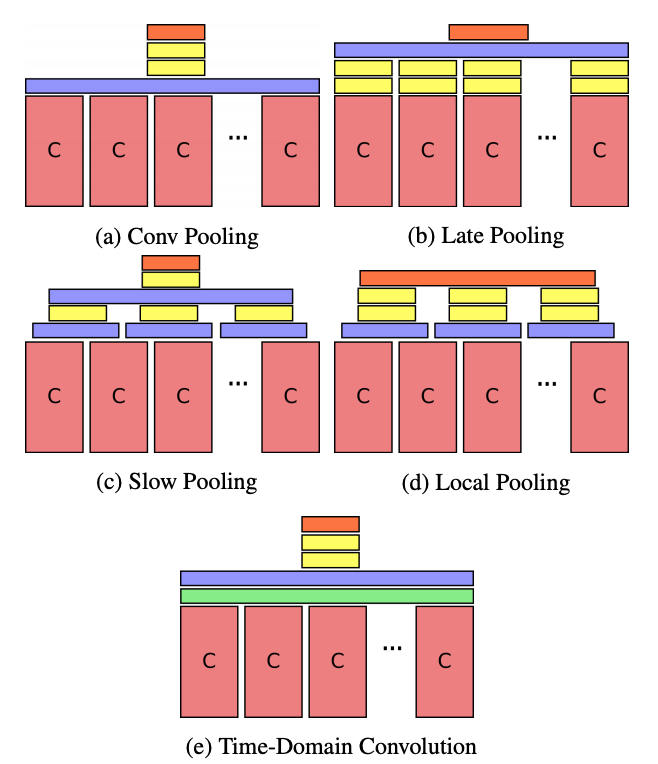
\includegraphics[width=0.7\linewidth]{img/stacked_conv.png}
\end{figure}

\section{教師あり、教師なし、半(弱)教師あり学習}
機械学習の手法には、
上記で説明したように、ラベルの貼られているデータセットを用いて学習することを教師あり学習と呼び、その反対で、データセットはあっても、そのデータセットの特性を示したラベルが与えられていない場合のデータセットを用いて学習することを教師なし学習と呼ぶ。本研究では、3Dの内視鏡生検画像データで、教師あり学習を行う際にラベルの貼られたデータが少ないことで精度向上が期待できないことから、教師なし学習で腫瘍か正常かの判別をつけられる学習方法を考える必要があった。ここで教師なし学習で画像の特徴を抽出する方法としてオートエンコーダがある。画像の場合におけるオートエンコーダの手法とは、ある画像から情報を圧縮する「エンコーダ」と言われる部分と、その圧縮した情報から画像を復元する「デコーダ」の二つからなる。入力とデコーダから復元された画像が同じ画像になるようにニューラルネットワークで学習させる。この学習の結果、潜在変数は似てる画像どうしで近い値になるように変化し、この分布を見れば画像の分類を教師ラベルがなくても、学習を行うことができる。本研究では、このオートエンコーダの派生である。Variational Autoencoderを利用した。これはオートエンコーダの「エンコーダ」と「デコーダ」は同じネットワーク構造であるが、データセットの潜在変数の分布が、正規分布になるような制約を加えて学習を行う手法である。こうすることでAutoencoderの潜在変数では分布の距離に意味なかったが、Variational Autoencoderでは正規分布に埋め込まれるため、画像の類似度を分布が表現することができるところが特徴である。Variational Autoencoderをまずは、2Dの画像に対して分布が正常と腫瘍の画像で変化するのかを確認した。さらに3次元画像でも解析することで3DCNNを用いて画像をエンコーダのネットワークを作り、潜在変数の空間を作ることで3次元画像特有の情報を抽出することができ、2次元画像だけでは判断できない、血管構造の乱れなどが認識できるようになると考えられる。
\section{組織透明化技術}
\section{レーザー顕微鏡による撮像}
\section{HE染色}
細胞組織の形態を観察するための病理染色ではヘマトキシリン・エオジン染色(HE染色)が一般的に用いられる。細胞核を青紫色に染色し、細胞質をピンク色に染色する。
\chapter{本研究の目的}
胃のがんの病理診断で見落とし(false negative)をなくすこと。

<課題>

- データが少ない
    - 8検体(アノテーションは3検体)の3D画像
- 教師ラベルは圧倒的に少ない
- 教師ラベルを完全に信用してはいけない。(ざっくりとしたアノテーションになっているから。)
- データ間のばらつきが激しい (染色条件によって大きく異なる。)
    - (メモ)だからといって、単に白黒で学習しても良くない。色情報が大切。
    - HE染色にした方が人間が見やすいし、事前学習できる。
- せっかく3D情報が取れるから、これの情報を生かしたい。
    - 3Dの画像差分といった画像処理または、BiLSTMなどのDeep Learning
- 胃と大腸と小腸がデータとして使えるので、それぞれのデータを利用(転移学習)できるのか?
- 医者に見せる時の可視化方法を検討する必要がある
- このソフトウェアを使う時のシステム全体を理解(ハードウェアとの連携)

<既存手法による解決方法>

- データが少量の時の学習法
    - DataAugmentation
    
 - 3D画像の畳み込みについて
 googleの論文

- 教師ラベルが曖昧である時の学習法
    - 半教師あり学習の先行研究

<提案の解決方法>
- データが少量かつ教師ラベルが曖昧である時の学習法
ある程度の画像処理と、教師ありと教師なしを混ぜ合わせた、半教師あり学習の組み合わせ学習を信頼度の重み付けを自由に調整できる可変方式による識別境界設計。

教師ラベルだけを学習するときのリスク
    - 完全に信頼できるとは限らない。(見落としなど)
    - 医師ごとに判断が異なる。
    - 過学習する。
    
教師なし学習だけのリスク
    - 正常と腫瘍を区別する境界を決定できない。
    - 色や輝度で大きな変化をする。


\section{現状の病理診断}
本研究の目的は、内視鏡生検を透明にして人工知能で癌を見落とさない診断方法を開発することである。組織透明化技術LUCIDを用いて検体を丸ごと透明化し、レーザー顕微鏡で観察することで、顕微鏡の解像度で検体の内部まで3次元情報として解析することができる。蛍光タンパク質や蛍光色素に対してほとんど褪色を示さないため、蛍光ラベルと併用して組織を観察することができる。透明化されたサンプルをレーザー顕微鏡で撮影すると、従来のカットする手法に換算して1000カットに相当する。得られる顕微鏡撮影像が従来の2,3カットに対して数百倍となるので、専門医が診断をするには負担が大きくなってしまう。したがって、人工知能が3次元画像を解析して病変を検知し専門医に提示することで病変の見落としリスク(false negative)がゼロになる診断支援システムを開発することが本研究の目的である。
\section{問題の解決方法}
\chapter{実験方法}
- 画像処理
    - 画像の特徴を検出する
手法
    - 円検出・楕円検出
    - optical flowによる三次元形状の変化検出
 結果
     - 正常の構造を検出した。パラメータの設計次第で6~8割の検出ができる。
     - 病変の3次元構造の乱れを検出した。
メリット
    - 教師データを作成しなくても良い。
デメリット
    - サンプルごとにパラメータ調整が必要になる
    - 
 

- ディープラーニングによる教師あり学習
手法
    - 2D画像のCNN
        - InceptionResNet
        - Xception
        - VGG19
        - VGG16
        - ResNet50
        - InceptionV3
        - InceptionResNetV2
        
    - 3D画像のCNN
        - 3D CNN 複数のネットワーク構造で検証
        - LSTM or GRU and 2DCNN
結果
メリット
デメリット

- ディープラーニングによる教師なし学習
手法
    - AutoEncoder
    - Variational AutoEncoder
    - Variational AutoEncoder with Gaussian Mixture Model
    - Generative Adversarial Networks
    
結果
メリット
デメリット

- ディープラーニングによる半教師あり学習
手法
結果
メリット
デメリット

- 複数の手法のメリットを生かした最終的な提案

学習結果の可視化
- 確信度マップ
- Grad-CAM

ホルマリン固定された生検検体を、LUCIDで透明化して

\section{画像処理による腫瘍検出手法}

\section{教師あり学習}
Xception, VGG19, VGG16, ResNet50, InceptionV3, InceptionResNetV2で教師あり学習を行った。いずれも一般物体認識で学習済みのモデルを転移学習する。

\chapter{結果}
\section{画像処理による腫瘍検出手法}
胃腺の管構造を認識することができれば、正常の場合は規則正しい円形になっていて、以上の場合は円形が乱れているという違いを検出することができる。楕円検出や円検出のアルゴリズムを
\begin{figure}[h]
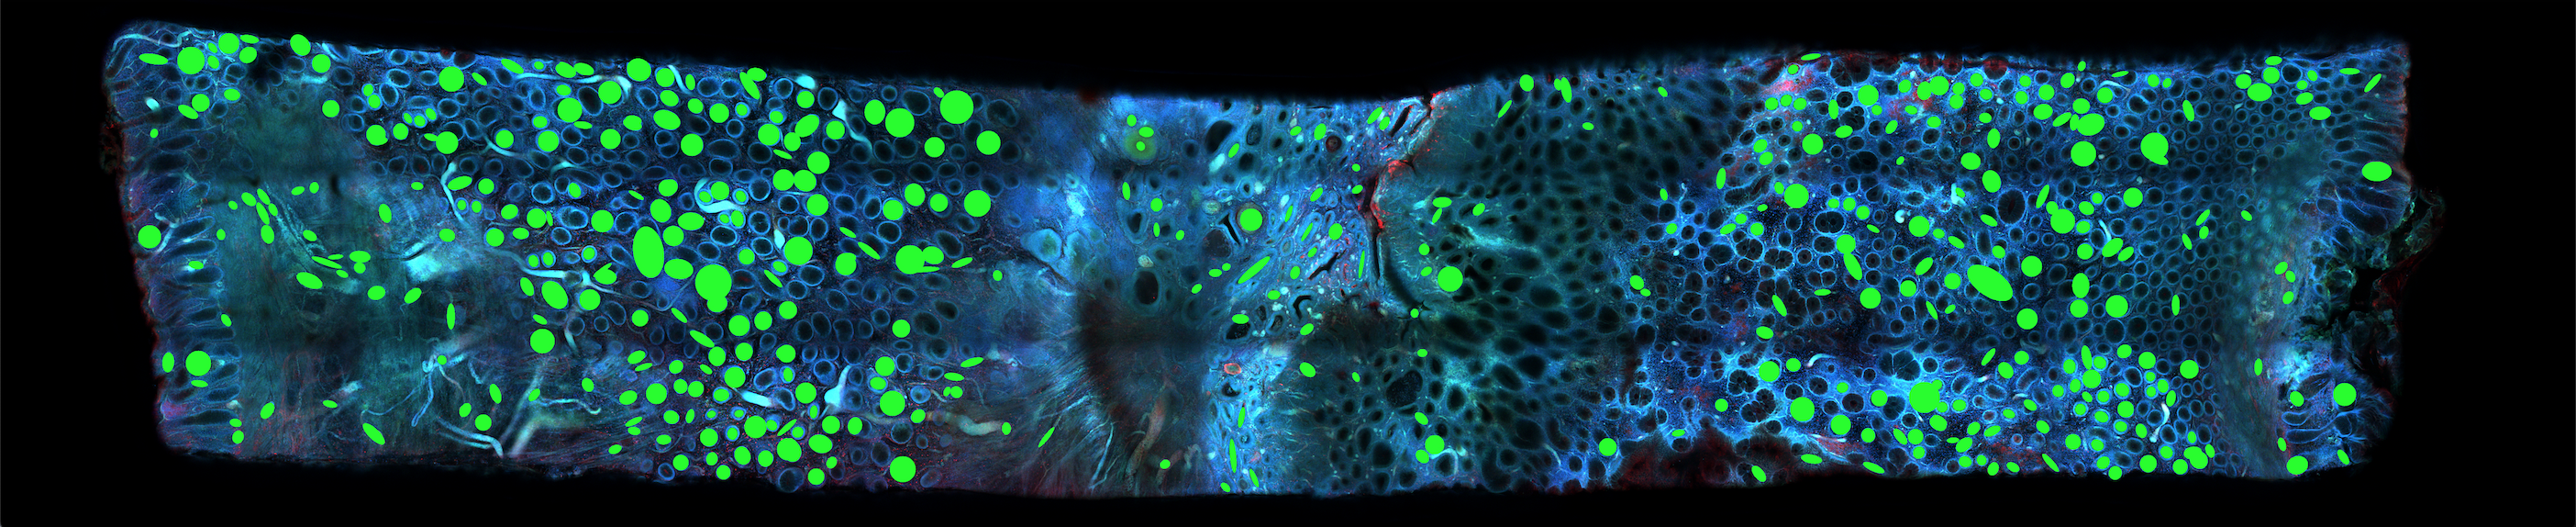
\includegraphics[width=15cm]{img/eclips_low.png}
\end{figure}
画像ごとにパラメータのチューニングが難しく現実的ではない。

\end{document}